%% !TEX program = xelatex
\documentclass[12pt, unicode]{beamer}
%\special{dvipdfmx:config z 0} %to uncompress and check
\special{pdf:minorversion 7} %set minorversion

\usepackage{fontspec}
\usepackage{polyglossia}
\setdefaultlanguage{russian}
\setotherlanguage{english}
\setsansfont{Fira Sans}
\newfontfamily\cyrillicfont{Fira Mono}
\renewcommand\UrlFont{\ttfamilylatin}

\usepackage{nicefrac}

\usepackage{lmodern}
\usepackage{graphicx}
\usepackage{multicol}
\usepackage{subcaption}
\usepackage{array}
\usepackage{calc}
\usepackage{colortbl}
\usepackage{tikz}
\usetikzlibrary{positioning,decorations,calc}
\graphicspath{{./images/}}
\usepackage{makecell}

\newcolumntype{C}[1]{>{\centering\arraybackslash}m{#1}}

\newif\ifstartcompletesineup
\newif\ifendcompletesineup
\pgfkeys{
    /pgf/decoration/.cd,
    start up/.is if=startcompletesineup,
    start up=true,
    start up/.default=true,
    start down/.style={/pgf/decoration/start up=false},
    end up/.is if=endcompletesineup,
    end up=true,
    end up/.default=true,
    end down/.style={/pgf/decoration/end up=false}
}
\pgfdeclaredecoration{complete sines}{initial}
{
    \state{initial}[
    width=+0pt,
    next state=upsine,
    persistent precomputation={
        \ifstartcompletesineup
        \pgfkeys{/pgf/decoration automaton/next state=upsine}
        \ifendcompletesineup
        \pgfmathsetmacro\matchinglength{
            0.5*\pgfdecoratedinputsegmentlength / (ceil(0.5* \pgfdecoratedinputsegmentlength / \pgfdecorationsegmentlength) )
        }
        \else
        \pgfmathsetmacro\matchinglength{
            0.5 * \pgfdecoratedinputsegmentlength / (ceil(0.5 * \pgfdecoratedinputsegmentlength / \pgfdecorationsegmentlength ) - 0.499)
        }
        \fi
        \else
        \pgfkeys{/pgf/decoration automaton/next state=downsine}
        \ifendcompletesineup
        \pgfmathsetmacro\matchinglength{
            0.5* \pgfdecoratedinputsegmentlength / (ceil(0.5 * \pgfdecoratedinputsegmentlength / \pgfdecorationsegmentlength ) - 0.4999)
        }
        \else
        \pgfmathsetmacro\matchinglength{
            0.5 * \pgfdecoratedinputsegmentlength / (ceil(0.5 * \pgfdecoratedinputsegmentlength / \pgfdecorationsegmentlength ) )
        }
        \fi
        \fi
        \setlength{\pgfdecorationsegmentlength}{\matchinglength pt}
    }] {}
    \state{downsine}[width=\pgfdecorationsegmentlength,next state=upsine]{
        \pgfpathsine{\pgfpoint{0.5\pgfdecorationsegmentlength}{0.5\pgfdecorationsegmentamplitude}}
        \pgfpathcosine{\pgfpoint{0.5\pgfdecorationsegmentlength}{-0.5\pgfdecorationsegmentamplitude}}
    }
    \state{upsine}[width=\pgfdecorationsegmentlength,next state=downsine]{
        \pgfpathsine{\pgfpoint{0.5\pgfdecorationsegmentlength}{-0.5\pgfdecorationsegmentamplitude}}
        \pgfpathcosine{\pgfpoint{0.5\pgfdecorationsegmentlength}{0.5\pgfdecorationsegmentamplitude}}
    }
    \state{final}{}
}

\tikzset{
    between/.style args={#1 and #2}{
        at = ($(#1)!0.5!(#2)$)
    }
}

\tikzset{
    between base/.style args={#1 and #2}{
        between=#1.base and #2.base
    }
}

\setbeamertemplate{note page}[plain]
%\setbeameroption{show notes on second screen=right}
%\setbeameroption{show only notes}

\newif\ifmetropolis
\metropolistrue

\title[Система автоматизированного A/B тестирования]{Система автоматизированного A/B~тестирования}
\author[Поликутин Е.Ю.]{
    \vbox{\raggedright%
        Студент группы М9119-09.04.01иибд ДВФУ\\ 
        Поликутин Евгений Юрьевич%
    }
    \vskip 20pt%
    \indent\vbox{\raggedright%
        Руководитель: Шевченко Игорь Иванович, к.т.н.\\
        Консультант: Олейников Игорь Сергеевич,\\ведущий аналитик данных ООО <<Амаяма Авто>>
        \ifmetropolis\else\vskip -0.5cm\fi%
    }
}
\date{10 июля 2021 г.}

\newif\ifPS
%\PStrue

\ifmetropolis
    \usetheme[progressbar=frametitle,numbering=fraction]{metropolis}
    \makeatletter
    \setlength{\metropolis@progressinheadfoot@linewidth}{2pt}
    \makeatother
\else
    \usetheme{CambridgeUS}
\fi

\setbeamersize{text margin left=3.5mm,text margin right=3.5mm} 

\newcommand{\pa}[1]{\left(#1\right)}

\usepackage{alphalph}
\makeatletter
\newcommand{\makeAlph}[1]{(\alphalph{\arabic{#1}})}
\makeatother

\newcommand*\rot{\rotatebox{90}}

\tolerance=1
\emergencystretch=\maxdimen
\hyphenpenalty=10000
\hbadness=10000

\begin{document}
    
    \frame{\thispagestyle{empty}\titlepage}
    
    \note{Защищается студент группы М9119-09.04.01иибд ДВФУ Поликутин Евгений Юрьевич по теме Система автоматизированного A/B тестирования. Научный руководитель --- кандидат технических наук Шевченко Игорь Иванович. Консультант --- ведущий аналитик данных ООО <<Амаяма Авто>> Олейников Игорь Сергеевич}
    
    \begin{frame}[fragile]{A/B тестирование}
    	\begin{figure}[h]
   			\centering
   			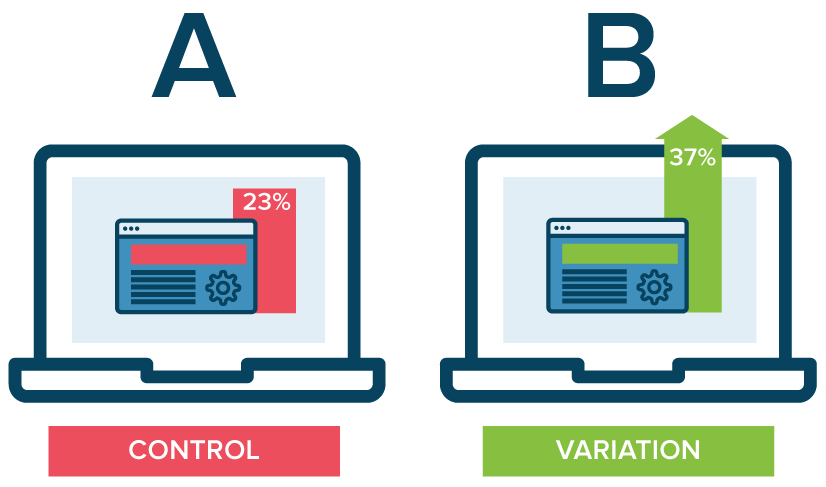
\includegraphics[width=0.9\textwidth]{ab_testing.png}
    	\end{figure}
    \end{frame}

	\note{A/B тестирование --- это статистический эксперимент, проводящийся путём разделения пользователей на 2 и более группы, представления им различных вариантов продукта и сравнением ключевых показателей. A/B тесты широко применяются как в веб-разработке, так и в разработке мобильных приложений, хотя основные статистические методы, применяемые в A/B тестировании, были сформулированы ещё около полувека назад для проведения медицинских клинических исследований}
	
	\begin{frame}[fragile]{\makebox(\framewidth,10){
\includegraphics[height=1cm]{drom_dark.pdf}\hfill}}
		\begin{block}{}
			\begin{itemize}
				\item 4 млн. посетителей в сутки (как в вебе, так и в приложениях)
				\item 450 млн. событий в сутки
				\item около 15 A/B тестов в месяц
			\end{itemize}
		\end{block}
	\end{frame}

	\note{
		<<Дром>> --- автомобильный портал, который также является "доской объявлений" о продаже автомобилей. Как портал, так и приложения постоянно дорабатываются, и возникает необходимость оценивать влияние вносимых изменений на ключевые метрики продуктов. Без А/Б тестирования достоверно это сделать практически невозможно, так как сезонные изменения, различные события (например, апрель 2020 года) и прочие факторы вносят искажения в вычисления.
	}

	\begin{frame}[fragile]{Цель и задачи работы}
		\begin{block}{Цель}
			\ifmetropolis
				\smallskip
			\fi
			Разработать и внедрить систему автоматизированного A/B тестирования в проекте <<Дром>>.
		\end{block}
		\begin{block}{Задачи}
			\begin{enumerate}
				\item Изучить преимущества и недостатки существующих систем A/B тестирования, таких как Firebase и Optimizely
				\item На основе данных обзора сформулировать требования к внедряемому решению
				\item Реализовать, внедрить и обеспечить освоение менеджерами разработанного решения
			\end{enumerate}
		\end{block}
	\end{frame}
	
	\note{
		Тесты проводились вручную, что занимало рабочее время аналитиков, и, тем самым, ограничивало либо количество проводимых тестов, либо их качество.
		\par Автоматизация A/B тестов позволила бы уменьшить нагрузку на аналитиков, увеличить количество проводимых тестов, ускорить процесс принятия решений и стандартизировать его; дала бы менеджерам возможность непосредственно участвовать в процессе A/B тестирования.
	}
    
    \begin{frame}[fragile]{Анализ существующих решений}
    	\color{black}
		\begin{table}[h]
			\centering\linespread{0.79}
			\begin{tabular}{|m{4cm}|c|c|c|c||c|c|c||c|c||c|}
			\hline
			& \rot{{\scriptsize Firebase\ }} & \rot{{\scriptsize Optimizely\ }} & \rot{{\scriptsize VWO\ }} & \rot{{\scriptsize Evergage\ }} & \rot{{\scriptsize Taplytics\ }} & \rot{{\scriptsize Countly\ }} & \rot{{\scriptsize Matomo\ }} & \rot{{\scriptsize Planout\ }} & \rot{{\scriptsize Sixpack\ }} & \rot{\shortstack{\scriptsize Разработанная\\ \scriptsize система}\ } \\
			\hline
			{\scriptsize мобильные приложения + веб} & 
			\textpm & + & + & + & + & + & + & \textminus & \textminus & + \\
			\hline
			{\scriptsize хостинг on-premises} &
			\textminus & \textminus & \textminus & \textminus & + & + & + & + & + & + \\
			\hline
			{\scriptsize анализ сырых данных} &
			+ & \textpm & \textpm & + & + & \textpm & \textpm & \textminus & \textminus & + \\
			\hline
			{\scriptsize гибкая настройка метрик} &
			\textminus & \textminus & \textminus & \textminus & \textminus & \textminus & \textminus & \textminus & \textminus & + \\
			\hline 
			{\scriptsize корректный непрерывный мониторинг тестов} &
			+ & + & + & + & + & + & \textminus & \textminus & \textminus & + \\
			\hline
			{\scriptsize самостоятельная доработка системы} &
			\textminus & \textminus & \textminus & \textminus & \textminus & + & + & + & + & + \\
			\hline
			{\scriptsize методики уменьшения дисперсии} &
			\textminus & \textminus & \textminus & \textminus & \textminus & \textminus & \textminus & \textminus & \textminus & + \\
			\hline
			{\scriptsize работа с существующими базами данных} &
			\textminus & \textminus & \textminus & \textminus & \textminus & \textminus & \textminus & \textminus & \textminus & + \\
			\hline
			\end{tabular}
		\end{table}
    \end{frame}

	\note{Большинство присутствующих на рынке программных продуктов для A/B тестирования являются облачными решениями для аналитики, требующими передачи данных на сервера других компаний; такой формат также не позволяет самостоятельно дорабатывать систему и добавлять новые метрики. Существующие же on-premises решения обладают слабым функционалом, а используемые СУБД не позволяют обрабатывать необходимый объём событий --- объём обрабатываемых данных меньше на порядок. Решения с исходным кодом позволяют только разделять пользователей на когорты, не содержат функционала анализа результатов.}
	
	\begin{frame}[fragile]{Краткие характеристики разработанной системы}
		\begin{block}{}
			\begin{itemize}
				\item 3300 строк на Python
				\item 300 строк на C++
				\item 1200 строк на TypeScript
				\item 10 модулей
				\item 4 страницы интерфейса
				\item FastAPI
				\item React
				\item Boost.Python
				\item Kubernetes
			\end{itemize}
		\end{block}
	\end{frame}

	\note{
		На <<Дроме>> уже существовала система управления A/B тестами (но не анализа результатов), поэтому разработка была сконцентрирована именно в области корректного мониторинга и анализа результатов тестов.
		\par Python был выбран для реализации как наиболее подходящий язык для задач анализа данных. Интерфейс был реализован на React.
		\par Система контейнеризована и разворачивается с помощью Kubernetes.
	}
	
	\begin{frame}[fragile]{Диаграмма компонентов}
		\begin{figure}[h]
			\centering
			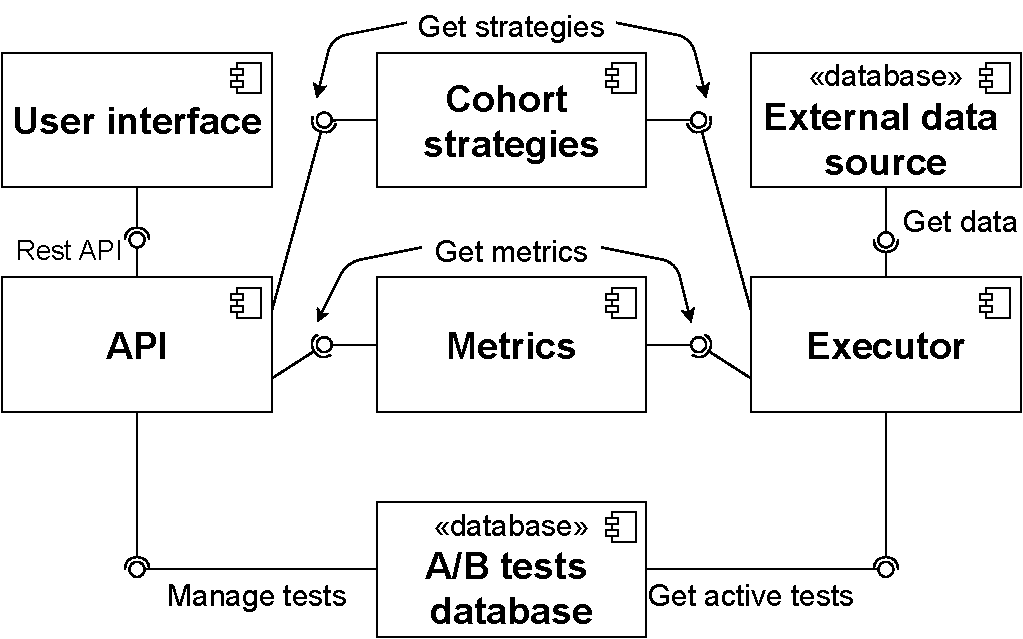
\includegraphics[width=0.75\textwidth]{component_diagram_big.pdf}
		\end{figure}
	\end{frame}
	
	\note{
		Архитектурно система состоит из Executor-a, исполняющего тесты по расписанию, и пользовательского интерфейса, через который осуществляется управление тестами и просмотр их результатов. Остальные части системы представляют собой их общие зависимости: метрики, стратегии разделения на когорты, база данных с результатами тестов, реализованные математические методы.
	}

	\begin{frame}[fragile]{Примеры метрик}
		\begin{block}{}
			\begin{itemize}
				\item Конверсия
				\item CTR (click-through rate)
				\item Среднее количество приобретённых платных услуг (на пользователя)
				\item Среднее количество потраченных денег (на пользователя)
				\item Заполняемость объявлений
			\end{itemize}
		\end{block}
	\end{frame}
	
	\note{
		На <<Дроме>> используется большое количество различных метрик, использующих различные базы данных. В связи с этим было принято решение вынести всю логику вычисления метрик в сами метрики, реализовав их как саморегистрирующиеся модули и взамодействуя с ними через интерфейс.
	}

	\begin{frame}[fragile]{Примеры стратегий\\ распределения пользователей на когорты}
		\begin{block}{}
			\begin{itemize}
				\item По последнему символу Ring (id пользователя)
				\item По последнему символу DeviceId (id устройства пользователя)
				\item По флагу от А/Б тестов Firebase (используется в мобильных приложениях)
				\item По значению hash-функции от id пользователя (в будущем)
			\end{itemize}
		\end{block}
	\end{frame}
	
	\note{
		Аналогично была решена схожая проблема со стратегиями распределения пользователей на когорты: на вебе пользователи, как правило, делятся по последнему символу случайно генерируемого id пользователя, в мобильных приложениях --- через флаги Firebase, а в будущем планируется переход на принятое в индустрии разделение по хэшу от id пользователя.
	}

	\begin{frame}[fragile]{Страница списка A/B тестов}
		\begin{figure}[h]
			\centering
			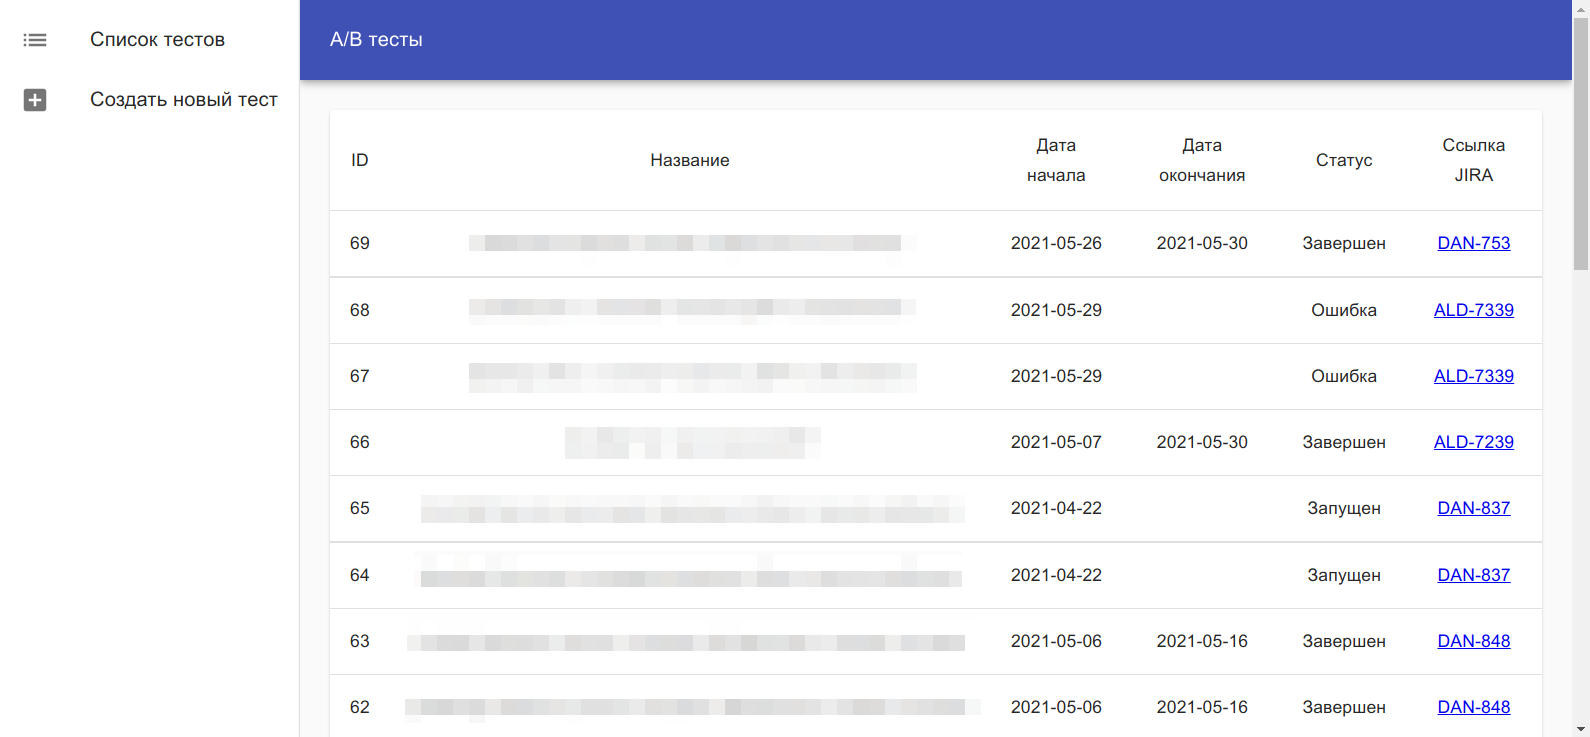
\includegraphics[width=\textwidth]{main_page.png}
		\end{figure}
	\end{frame}
	
	\note{
		Интерфейс примерно повторяет интерфейсы существующих систем и позволяет создавать, изменять, просматривать результаты и управлять A/B тестами.
	}

	\begin{frame}[fragile]{Страница результата A/B теста}
		\begin{figure}[h]
			\centering
			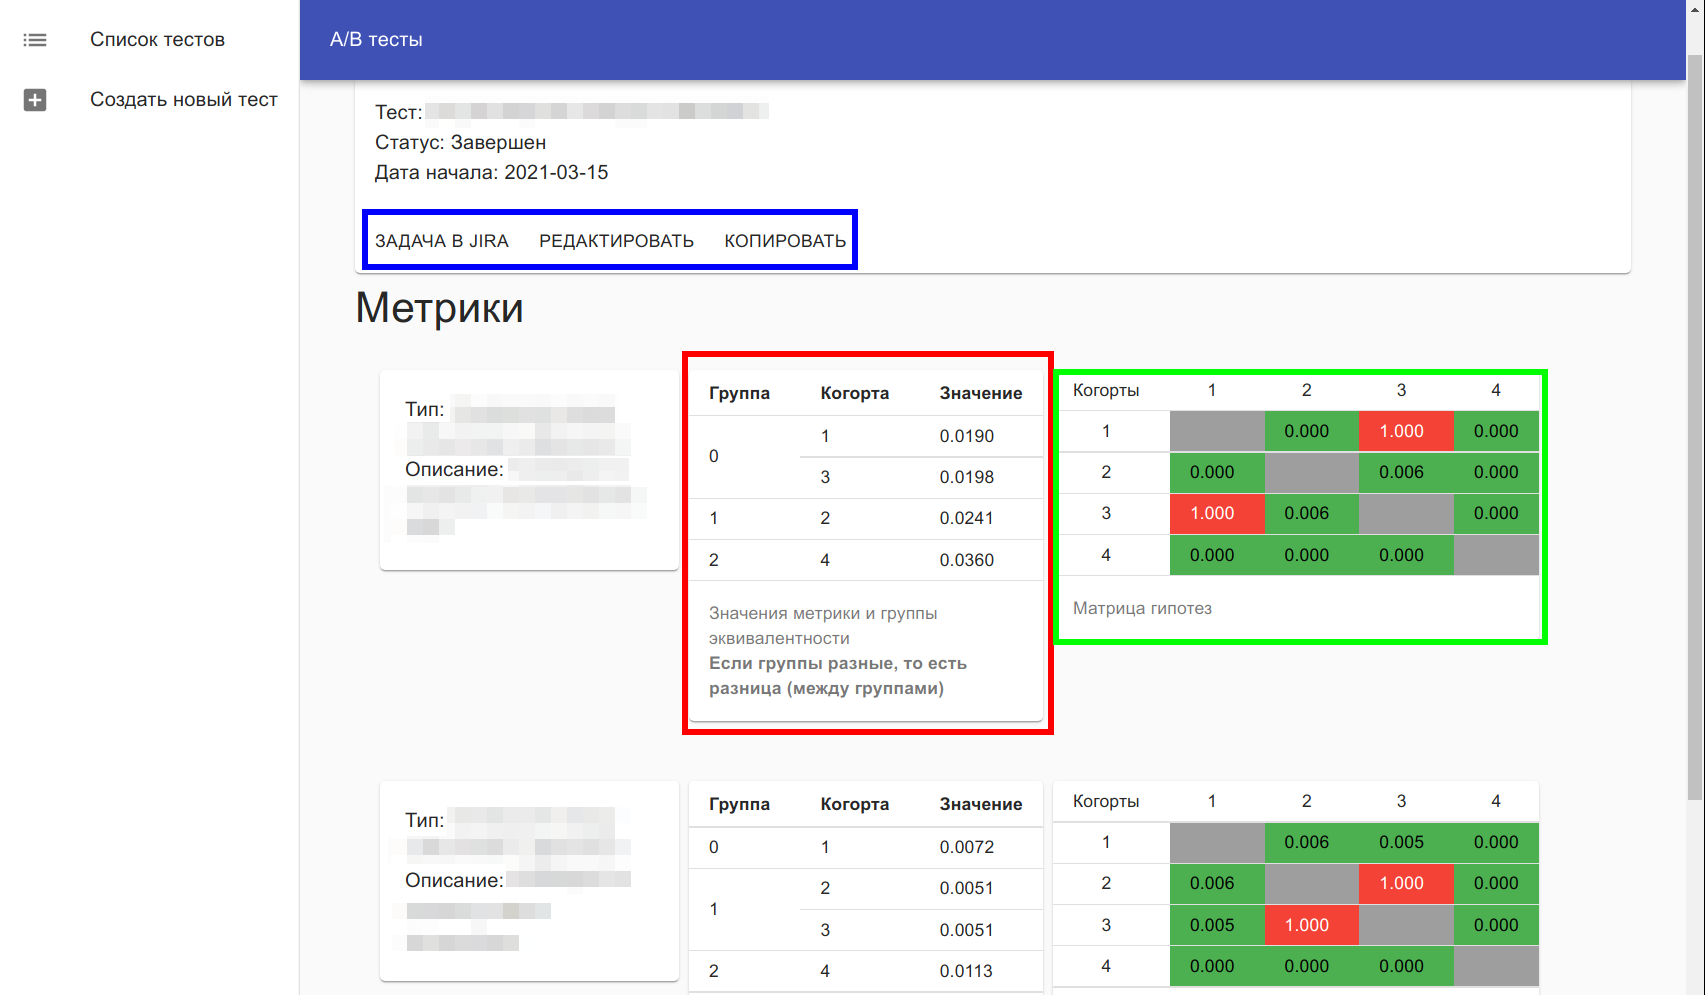
\includegraphics[width=\textwidth]{test_page.png}
		\end{figure}
	\end{frame}
	
	\note{
		Отображение результатов теста является нетривиальной задачей, так как в тесте может участвовать более 2 когорт пользователей. Для её решения в интерфейсе выводятся значения p-value для каждой пары когорт (выделено зелёным), скорректированные для ситуации множественного сравнения, а также группы эквивалентности когорт, полученные в результате использования системы непересекающихся множеств (выделено красным). Также отображены (и выделены синим) кнопки управления тестом.
	}

	\begin{frame}[fragile]{Генерация формы редактирования A/B теста}
		\begin{block}{}
			\begin{itemize}
				\item pydantic генерирует JSONSchema для A/B теста, метрик и стратегий распределения
				\item Схема A/B теста дополняется схемами метрик и стратегий распределения
				\item Форма отрисовывается с помощью библиотеки react-jsonschema-form
			\end{itemize}
		\end{block}
	\end{frame}
	
	\note{
		В связи с модульностью было принято решение генерировать форму создания и редактирования теста автоматически, используя схемы параметров метрик и распределений по когортам. Для этого JSONSchema генерируется с помощью библиотеки pydantic из структур на Python, дополняется для поддержки условных выражений для отображения параметров метрик/стратегий только для соответствующих пунктов списков и отображается с помощью библиотеки react-jsonschema-form.
	}

	\begin{frame}[fragile]{Статистическая формулировка A/B теста}
		\begin{block}{}
			\vspace*{-0.8cm}
			\begin{equation*}
				\begin{aligned}
					&H_0:\ \overline{X}=\overline{Y}\\
					&H_1:\ \overline{X}\ne\overline{Y}\\
					&P(\text{отвергнуть}\ H_0|H_0\ \text{верна})=\alpha\\
					&P(\text{отвергнуть}\ H_0|H_1\ \text{верна})=1-\beta\\
					&p = P(\text{наблюдать }\overline{X}-\overline{Y}\ |H_0\ \text{верна})\\
					&p<\alpha\Rightarrow\text{разница статистически значима}
				\end{aligned}
			\end{equation*}
			\vspace*{-0.5cm}
			\begin{itemize}
				\item $\overline{X},\ \overline{Y}$ --- средние значения в 2 когортах A/B теста
				\item $H_0,\ H_1$ --- нулевая и альтернативная гипотезы
				\item $\alpha$ --- уровень значимости
				\item $1-\beta$ --- статистическая мощность
				\item $p$ --- p-value
			\end{itemize}
		\end{block}
	\end{frame}
	
	\note{
		А/Б тест формулируется как статистический эксперимент, в котором, как правило, сравниваются средние значения метрики двух когорт A/B теста, и отвергается, или не отвергается, нулевая гипотеза о равенстве этих средних. В классическом А/Б тестировании результаты считаются 1 раз, по достижению необходимого количества пользователей в когортах.
	}

	\begin{frame}[fragile]{Проблема подглядывания}
		\begin{figure}
			\centering
			\begin{minipage}{0.5\textwidth}
				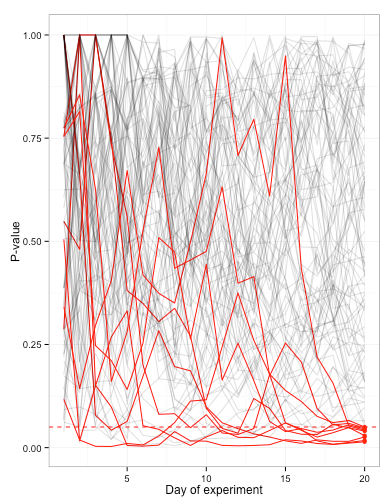
\includegraphics[width=0.9\textwidth]{p_values_correct.png}
				\caption{Корректный тест}
			\end{minipage}%
			\begin{minipage}{0.5\textwidth}
				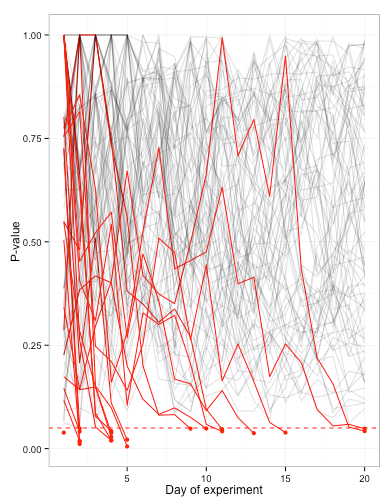
\includegraphics[width=0.9\textwidth]{p_values_peeking.png}
				\caption{Тест с подглядыванием}
			\end{minipage}
		\end{figure}
	\end{frame}
	
	\note{
		Проблема подглядывания возникает тогда, когда p-value считается несколько раз за время теста, и тест останавливается по пересечению уровня значимости. Это приводит к значительному росту вероятности ошибок 1 рода --- обнаружению эффекта там, где его в действительности нет. На рисунках изображены 5000 симулированных A/B тестов в условиях отсутствия реального эффекта. Легко видеть, что справа ложноположительных срабатываний больше --- не 5, а целых 22 процента.
	}
	
	\begin{frame}[fragile]{mSPRT\footnote[1]{Johari et al, 2017
			} --- mixture sequential probability ratio test}
		\begin{block}{}
			\vspace*{-0.8cm}
			\begin{equation*}
				\begin{aligned}
					\Lambda_{n}^{H,\theta_0}=\int_{\Theta}\prod\limits_{m=1}^{n}\frac{f_{\theta}(Z_m)}{f_{\theta_0}(Z_m)}h(\theta)\mathrm{d}\theta\\
					p_0=1;\;p_n=\min\{p_{n-1},1/\Lambda_{n}^{H,\theta_0}\}
				\end{aligned}
			\end{equation*}
			\vspace*{-0.5cm}
			\begin{itemize}
				\item $\theta$, $\theta_0$ --- целевой параметр, например, разница средних и его значение при нулевой гипотезе
				\item $f_{\theta}$ --- функция правдоподобия параметра $\theta$ (плотность распределения разности $Z=X-Y$)
				\item $h$ --- плотность смешивающего распределения
				\item $Z_m$ --- элемент данных, $Z_m = X_m - Y_m$ в контексте A/B теста
				\item $p_i$ --- p-value на шаге $i$
			\end{itemize}
			\vspace*{-0.5cm}
		\end{block}
		\vfill\null
	\end{frame}

	\note{
		Для избежания проблемы подглядывания в работе применяется критерий mSPRT, специально предназначенный для такого сценария, и его модификации. Для этого теста играет роль выбор смешивающего распределения, которое играет роль априорной оценки эффекта теста.
	}
	
	\begin{frame}[fragile]{mSPRT для разности средних при нормальном распределении метрики\footnote[1]{Johari et al, 2017
		}}
		\begin{block}{}
			\begin{equation*}
				\begin{aligned}
					\Lambda_{n}^{H} = \sqrt{\frac{2\sigma^2}{2\sigma^2 +n\tau^2}} \exp\left\{\frac{n^2\tau^2 (\overline{Y}_n-\overline{X}_n)^2}{4\sigma^2(2\sigma^2+n\tau^2)}\right\}\\
					p_0=1;\;p_n=\min\{p_{n-1},1/\Lambda_{n}^{H}\}
				\end{aligned}
			\end{equation*}
			\vspace*{-0.5cm}
			\begin{itemize}
				\item $\sigma$ --- стандартное отклонение объединённой выборки
				\item $n$ --- объём объединённой выборки
				\item $\tau$ --- ожидаемый размер эффекта
				\item $\overline{X}_n,\ \overline{Y}_n$ --- средние двух популяций A/B теста
				\item $p_i$ --- p-value на шаге $i$
			\end{itemize}
			\vspace*{-0.5cm}
		\end{block}
		\vfill\null
	\end{frame}
	
	\note{
		Этот критерий требует знания точной формы распределения --- например нормальное, или Бернулли --- в этих случаях формула выражается в аналитическом виде и может быть легко применена. Смешивающее распределение в таком случае так же берётся нормальным c центром в 0 и дисперсией тау-квадрат.
	}

	\begin{frame}[fragile]{Bootstrap mSPRT\footnote[1]{
				Abhishek V. et al, 2017
		}}
		\begin{block}{}
			\begin{itemize}
				\item распределение данных заранее неизвестно
				\item функция правдоподобия заменяется эмпирической оценкой по данным
				\begin{itemize}
					\item бутстрап
					\item KDE (ядерная оценка плотности)
					\item интеграл берётся методом Монте-Карло
				\end{itemize}
				\item полезно для метрик, связанных с покупками пользователей
				\begin{itemize}
					\item среднее количество приобретённых услуг
					\item средний доход на пользователя
				\end{itemize}
			\end{itemize}
		\end{block}
		\vfill\null
	\end{frame}

	\note{
		Однако в случае с некоторыми метриками, особенно связанными с финансами, функция правдоподобия в аналитическом виде неизвестна. Для анализа таких метрик применяется модификация данного метода, которая эмпирически оценивает функцию правдоподобия по данным с помощью бутстрапа и ядерной оценки плотности, и берёт интеграл, используя метод Монте-Карло.
	}

	\begin{frame}[fragile]{Уменьшение дисперсии\footnote[1]{
				A. Poyarkov et al, 2016
			} с помощью CatBoost\footnote[2]{A.V. Dorogush et al, 2017}}
		\begin{block}{}
			\vspace*{-0.8cm}
			\begin{equation}
				\begin{aligned}
					\tilde{Y}&=F(X)\\
					Y^*&=Y-\tilde{Y}\\
					Y^*_1 - Y^*_2 = \text{ATE}(Y^*)&=\text{ATE}(Y)=Y_1 - Y_2 \\
					\text{var}(Y^*)&=\text{var}(Y)-\text{var}(\tilde{Y})
				\end{aligned}
			\end{equation}
			\vspace*{-0.5cm}
			\begin{itemize}
				\item $X$ --- некоторые предэкспериментальные данные
				\item $Y$ --- наблюдаемые значения метрики
				\item $\tilde{Y}$ --- предсказанные значения метрики
				\item ATE --- средний эффект изменений
				\item var --- дисперсия
			\end{itemize}
		\end{block}
		\vfill\null
	\end{frame}
	
	\note{
		Для уменьшения времени проведения теста, а, следовательно, ускорения принятия решений менеджерами используется метод уменьшения дисперсии на основе градиентного бустинга. В качестве алгоритма бустинга был выбран CatBoost. Предсказания с его использованием значения метрики для каждого пользователя на основе предэкспериментальных данных позволяют объяснить часть дисперсии и снизить влияние сторонних факторов на эксперимент. При этом разница метрики между когортами остаётся неизменной.
		\par Уменьшение дисперсии подобным образом особенно полезно для метрик, связанных с пользовательскими покупками: пользователи, покупавшие услуги в прошлом, более вероятно воспользуются ими в будущем; чем больше услуг покупает пользователь до теста, тем больше он приобретёт во время теста.
	}

	\begin{frame}[fragile]{Итоги}
		\begin{itemize}
			\item Успешно разработана и внедрена система автоматизированного A/B тестирования на проекте <<Дром>>
			\item Перестроены процессы проведения A/B тестов
			\item Качество A/B тестов повысилось
			\item Система положительно принята менеджерами продуктов
			\item На текущий момент менеджерами с использованием системы было проведено 75 A/B тестов, чем сэкономлено около 600 часов работы аналитиков
		\end{itemize}
	\end{frame}

	\note{
		В результате проведённой работы была 
		\begin{itemize}
			\item успешно разработана и внедрена система автоматизированного A/B тестирования
			\item перестроены процессы проведения A/B тестов --- аналитики только следят за корректностью методики, а продакт-менеджеры проводят их самостоятельно
			\item качество A/B тестов повысилось в результате систематизации работы с ними, для исключения ошибок тесты с новыми метриками перепроверяются аналитиками вручную
			\item значительно сэкономлено рабочее время аналитиков данных
		\end{itemize}
		\par Доклад окончен, спасибо за внимание.
	}
    
\end{document}